This section is dedicated to understand the performance of the proposed \ac{JSFRA} scheme with different values of \me{\ell_q} over multiple time slots. The performance is compared with the existing \ac{Q-WSRME} scheme for different arrival rates \me{A_k}. Fig. \ref{fig-review} compares the performance of the centralized algorithms for different \me{\ell_q} values using the average number of backlogged packets present in the system after each time instant. The horizontal axis indicate the average arrivals in bits per user, which is constant for all user. The instantaneous arrival follows Poisson distribution. The model considered for simulation is a \me{4 \times 1} \ac{MIMO} system with \me{N = 4} sub-channels with \me{N_B = 2} \acp{BS}. The path loss is modeled as a uniform random variable \me{[0,-3]} dB with the maximum \ac{SINR} seen by any user is \me{6} dB. The average is performed over \me{100} time slots.
\begin{figure}
	\centering
	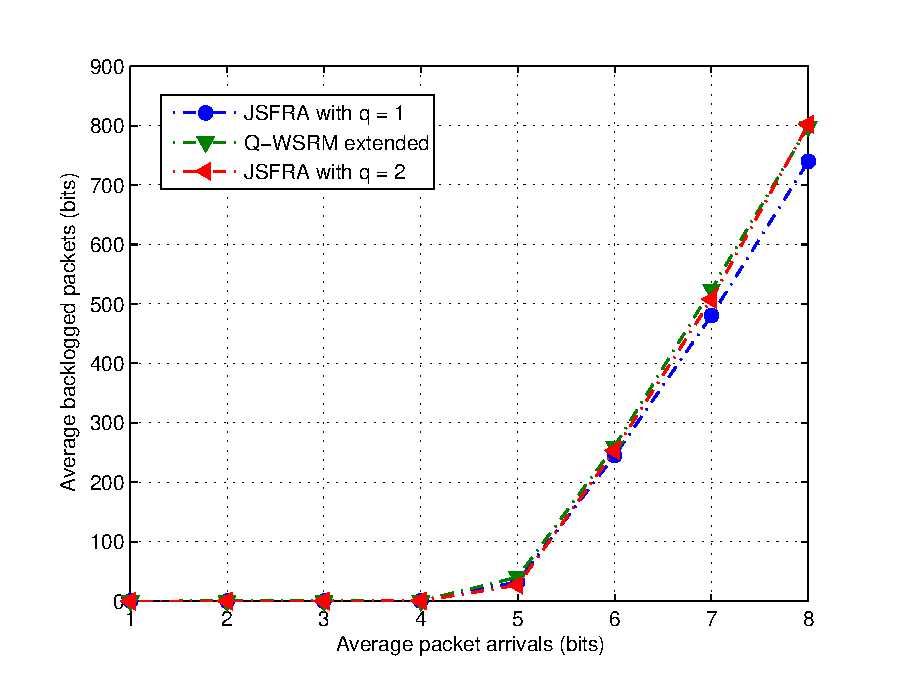
\includegraphics[width=\columnwidth]{Review/reviewer.eps}
	\label{fig-review}
	\caption{System \me{\lbrace N,N_B,K,N_R \rbrace = \lbrace 4,2,12,1 \rbrace}}
\end{figure}

It can be seen from Fig. \ref{fig-review} that the performance of the \ac{JSFRA} scheme with \me{\ell_2} norm and the \ac{Q-WSRME} approach are similar in the average residuals after each transmission instant. Note that the performance of the \ac{Q-WSRM} scheme is similar to the \ac{Q-WSRME} approach when the arrival rates are greater than the actual transmissions. It can be seen from Fig. \ref{fig-review} that the average number of backlogged packets are contained until the per user arrival is \me{\leq 4} bits. After that, the average queues become unbounded. The performance of the \ac{JSFRA} scheme with \me{\ell_1} norm has significantly less number of average queued packets in comparison with other schemes. The performance of the \ac{JSFRA} scheme with \me{\ell_{\infty}} performs the worst in terms of the average number of queued packets after each transmission instant by achieving the fair service rate to all users.
